% -- Document configuration
\documentclass{article}

% -- Input and language settings
% \usepackage[utf8]{inputenc}
\usepackage[spanish]{babel}
\decimalpoint                             % From babel package to use points instead of commas in decimals

% -- Page and line settings
\usepackage{geometry}
\geometry{letterpaper, 
    % margin=2cm, 
    left=3cm, right=3cm,
    top=1.2cm, bottom=1.2cm,
    includefoot, 
    includehead}
\renewcommand{\baselinestretch}{1.2}

% -- Required packages
\usepackage{xcolor}
\usepackage[many]{tcolorbox}
\usepackage{mathtools,amsfonts,amsmath}     % Loads amsmath if not already loaded
\allowdisplaybreaks                         % To allow page breaks if equations are too long
\usepackage[parfill]{parskip}               % No indent and separation lines for paragraphs
\usepackage{cancel}                         % To cancel math terms
\usepackage[shortlabels]{enumitem}          % To handle enumerations
\usepackage{tikz}
\usetikzlibrary{automata, arrows.meta, positioning}
\usepackage[mode=buildnew]{standalone}      % To import figures in standalone files
\usepackage[hidelinks]{hyperref}
\usepackage[spanish]{cleveref}              % To use autocompleted reference labels, language must be change as in babel package
\usepackage{caption}                        % Caption and subcaption to allow subfigures
\usepackage{subcaption}
\usepackage{float}                          % To specify the location of figures
\usepackage{multicol}                       % To use multicolumns
\usepackage[bottom]{footmisc}               % To locate footnotes at the bottom

% -- Title and heading settings
\usepackage{titling}
\usepackage{fancyhdr}
\pagestyle{fancy}

% -- Code and code formatting
\usepackage{minted}                         % To insert code
\usemintedstyle[julia]{gruvbox-light}       % Code theme and language
\definecolor{bg}{rgb}{0.98, 0.97, 0.88}     % Code block background

\usepackage{fontspec}                       % To allow the use of monospace fonts
\setmonofont{JuliaMono}[Path=./codefonts/, Extension=.ttf, UprightFont=*-Regular, ItalicFont=*-RegularItalic, Scale=0.75]

\usepackage{fancyvrb}                       % To change line number font
\renewcommand{\theFancyVerbLine}{\textcolor{gray}{\footnotesize\texttt{\arabic{FancyVerbLine}}}}

\definecolor{light-gray}{gray}{0.95}        % Color, box and style to show small code thingys inside normal text
\newcommand{\code}[1]{\colorbox{light-gray}{\texttt{#1}}}

% -- Bilbiography preferences
\usepackage[square,numbers]{natbib}
\bibliographystyle{unsrt}

% -- Footnotes without numbering
\newcommand\nnfootnote[1]{%
  \begin{NoHyper}
  \renewcommand\thefootnote{}\footnote{#1}%
  \addtocounter{footnote}{-1}%
  \end{NoHyper}
}

% -- Theorems
\newtheorem{theorem}{Theorem}

\lhead{\theinstitution\ -- \thedepartment}
\chead{}
\rhead{Programación para la IA\ -- \thetitle}
\lfoot{}
\cfoot{\thepage}
\rfoot{}

% -- Problem solution
\newenvironment{solution}
{\begin{quote}
\textbf{Solución:}\medskip

}
{

\hfill\rule{0.5\textwidth}{0.5pt}
\end{quote}}

% -- Equation result
\newcommand{\result}[1]
{
\tcbhighmath[colframe=white, colback=gray!15, sharp corners]
{#1}
}

% -- Function definitions
\newcommand{\dprod}[2]{{#1} \cdot {#2}}
\newcommand{\txtgray}[1]{\textcolor{gray}{#1}}

% -- Author information
\title{Actividad 5}
\author{Leonardo Flores Torres}
\newcommand\theinstitution{Universidad Veracruzana}
\newcommand\thedepartment{Inteligencia Artificial}
\newcommand\thecourse{Programación para la Inteligencia Artificial}

% -- Paths
% \newcommand\codelists{../programs/lists.rkt}

% Remove red color boxes of "syntax errors" in minted
\AtBeginEnvironment{minted}{%
  \renewcommand{\fcolorbox}[4][]{#4}}

\newcommand{\diannao}{\texttt{diannao}}
\newcommand{\hongdiannao}{\texttt{hongdiannao}}

% -- Document
\begin{document}

\thispagestyle{empty}

%Title
\begin{center}
\textsc{\theinstitution}\\[2mm]

\thedepartment

\rule{0.6\textwidth}{0.5pt}\\[2mm]

\thecourse \\[4mm]

{\Large \textbf{\thetitle}}\\[2mm]

\theauthor \\[2mm]

{\small \today}
\end{center}
\medskip

% -- 
\vspace{1cm}

\textbf{%
Programar un algoritmo de su elección (no tan sencillo) y analizarlo de la siguiente forma:}
\begin{enumerate}
    \item Graficar el tiempo de ejecución en función de $N$,
    \item sobre los mismos ejes graficar 2 cotas superiores y dos cotas inferiores,
    \item repetir el punto 1 y 2 ejecutando el programa en otra computadora de distinto desempeño,
    \item analizar los resultados y discutirlos. Escribir de la manera más completa las características de las 2 computadoras.
\end{enumerate}

\vspace{1cm}

El algoritmo que se eligió fue computar un fractal, más específicamente, el ...

El extracto de código que se muestra a continuación es una representación del modo de trabajo que se lleva en \code{julia} usando el REPL\footnote{REPL es un acrónimo para Read-Eval-Print loop.}, asemeja un ambiente de trabajo y ejecución de comandos en la terminal.
\begin{listing}[ht!]
    \begin{minted}[
        frame=none,
        % obeytabs=false,
        breaklines,
        tabsize=4,
        % linenos=true,
        % numbersep=-10pt,
        baselinestretch=1,
        firstnumber=last,
        bgcolor=bg,
    ]{julia}
    julia> ns = 10:10:400                       # valores que puede tomar N
    julia> reps = 10                            # numero de repeticiones
    julia> timings = zeros(length(ns), 2)       # arreglo bidimensional
    julia> for rep in 1:reps
                for (index, n) in enumerate(ns)
                    time = @elapsed mf.fractalCMap(n, n, maxiter=100)
                    if rep == 1
                        timings[index, 1] = n
                    end
                    timings[index, 2] += time
                end
            end
    julia> timings[:,2] = timings[:,2] / reps   # promedio de tiempo
    \end{minted}
\end{listing}

Para graficar el tiempo de ejecución se hicieron 10 repeticiones indicadas por \code{reps}, y se definió una variable \code{ns} para guardar el conjunto de valores que puede tomar $N = 10,\ 20,\ 30,\ \ldots,\ 400$. La variable \code{timings} guarda en la primera columna el valor de $N$, mientras que en la segunda columna guarda el tiempo $t(N)$ que le toma al algoritmo computar el fractal. Cada iteración del \code{loop} se suman los tiempos $t(N)$ a sus respectivas entradas, y al final toda la columna de tiempos se divide entre la cantidad de repeticiones \code{reps} lo que resulta en tiempos promedio $\tilde{t}(N)$.

Las características de las computadoras usadas, {\diannao} y {\hongdiannao}, se muestran en la \cref{fig:diannao-specs,fig:hongdiannao-specs}, respectivamente.
\begin{figure}[ht!]
    \centering
    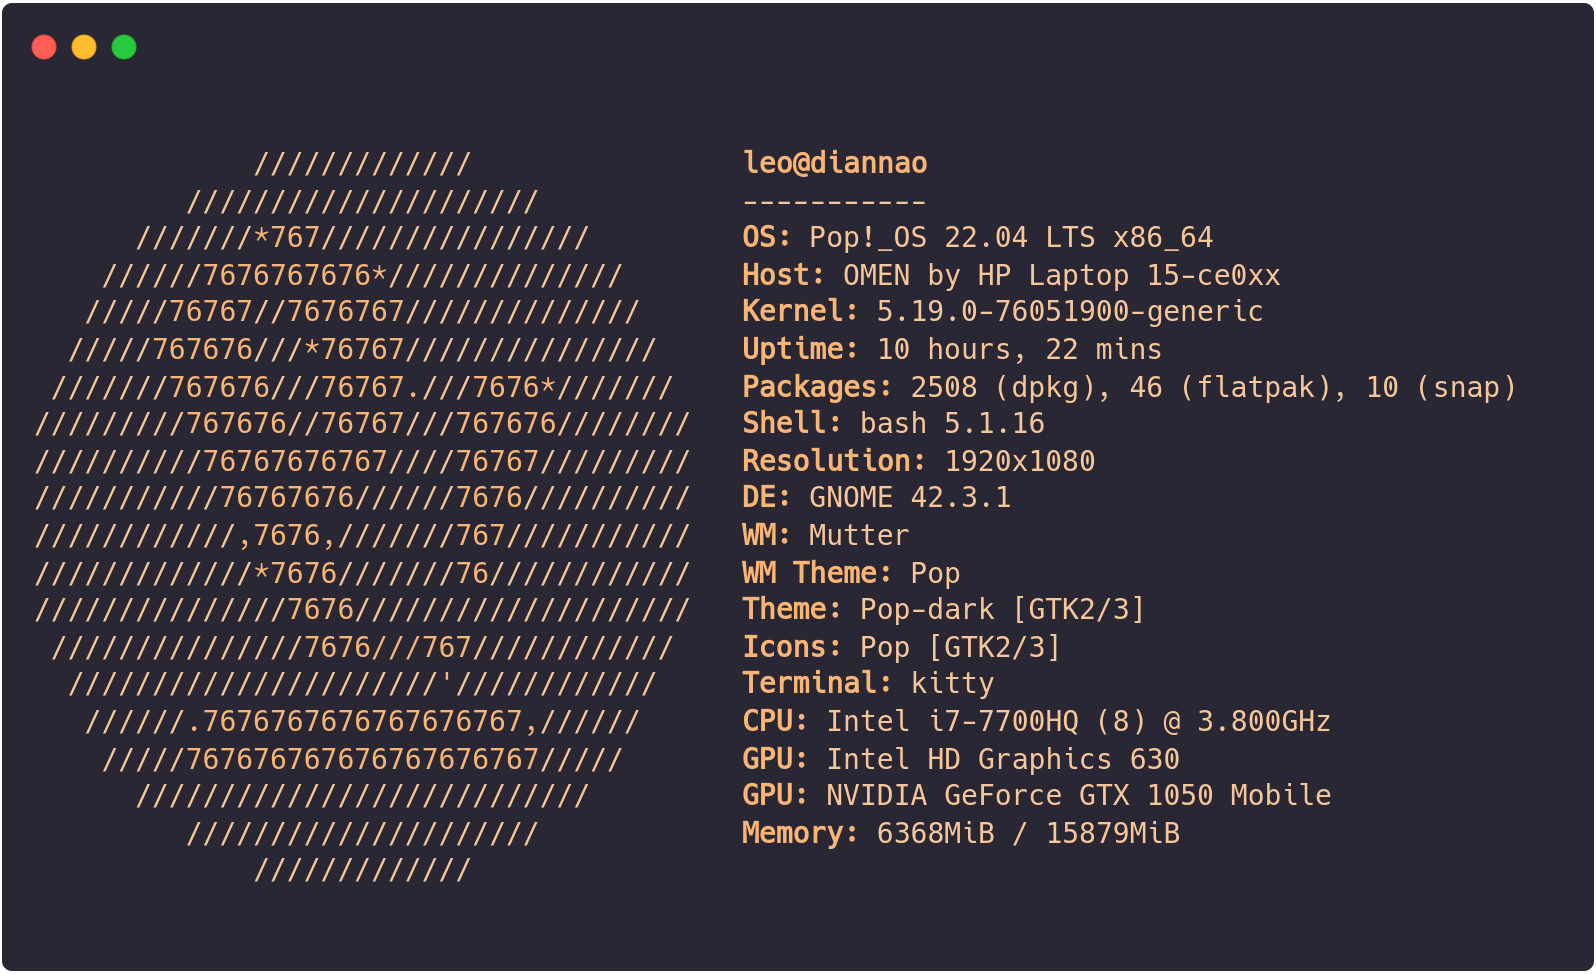
\includegraphics[scale=0.23]{../figures/diannao-specs}
    \caption{características del ordenador {\diannao}.}
    \label{fig:diannao-specs}
\end{figure}
\begin{figure}[ht!]
    \centering
    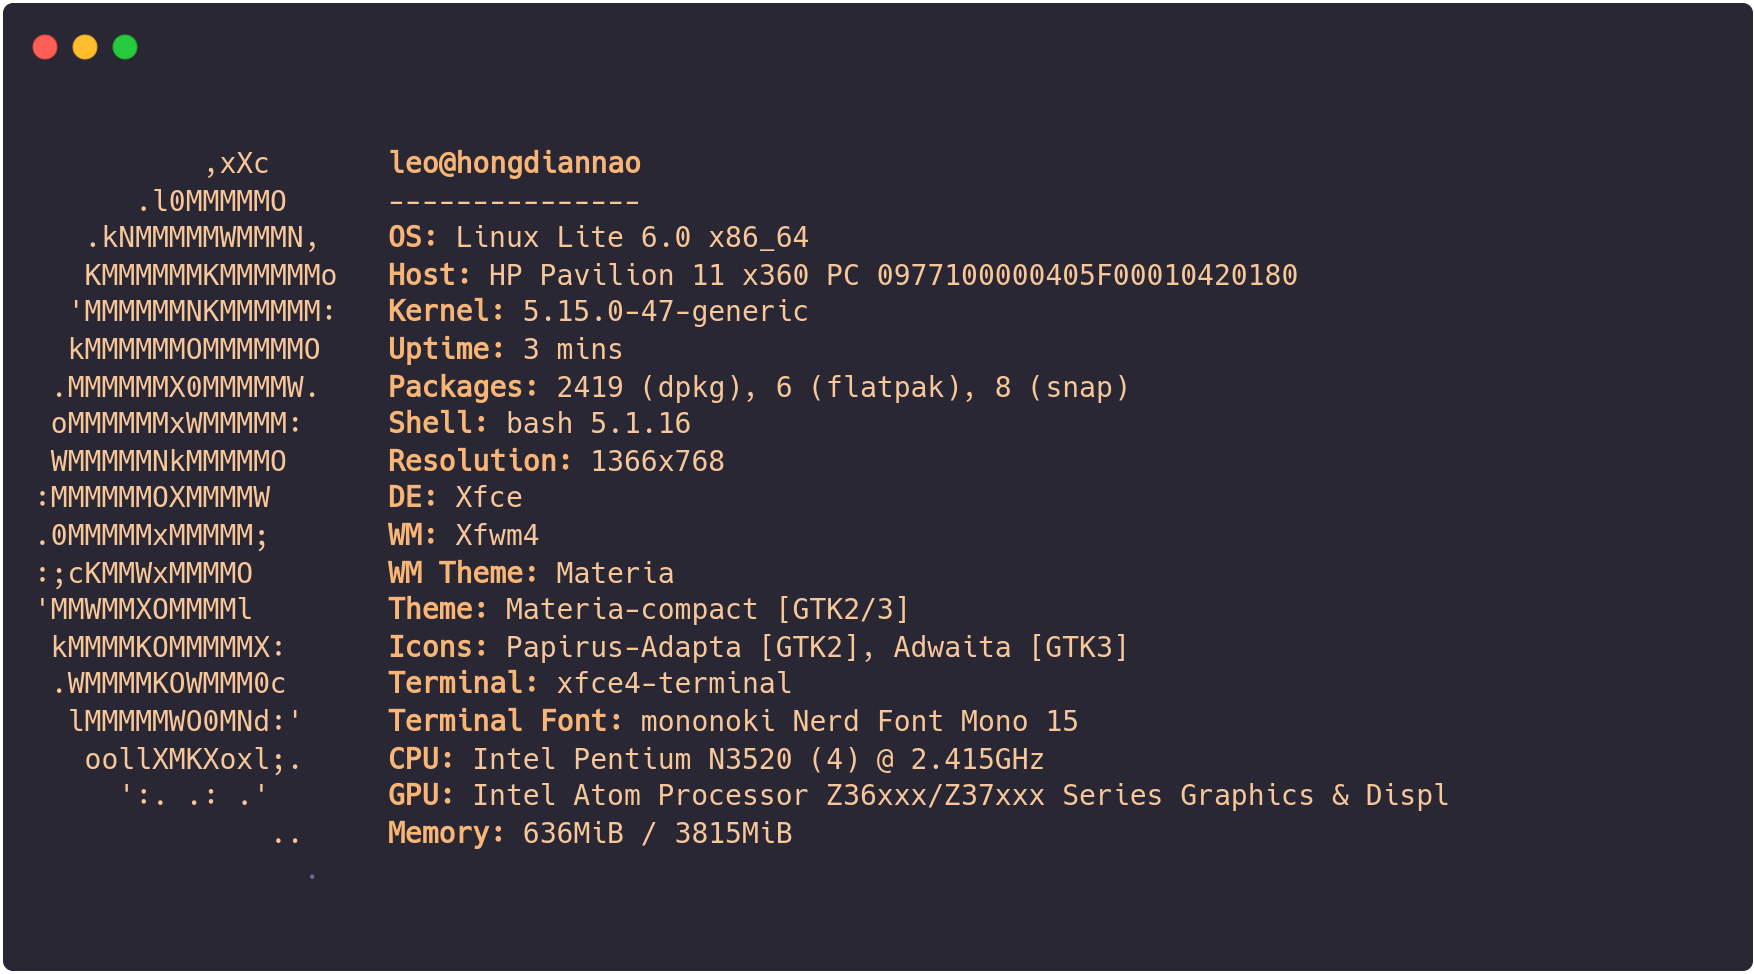
\includegraphics[scale=0.23]{../figures/hongdiannao-specs}
    \caption{características del ordenador {\hongdiannao}.}
    \label{fig:hongdiannao-specs}
\end{figure}

% \pagebreak
% -- BIBLIOGRAFIA
% \nocite{*} % to call all references even if they are not cited in the text
% \bibliography{references.bib}

\pagebreak
% -- CODIGO
\vspace{1cm}
\section*{Apéndice}
\inputminted[
    frame=none,
    % obeytabs=false,
    breaklines,
    tabsize=4,
    linenos=true,
    % numbersep=-10pt,
    baselinestretch=1,
    firstnumber=last,
    bgcolor=bg,
]{julia}{\codepath}


\end{document}